\subsection{Accelerometeralgoritme}
For at teste accelerometeralgoritmen sammenlignes de målte spændinger for accelerometrene, der er illustreret på \autoref{fig:test_femur_tibia} med vinklen af accelerometrene.
Testen, der illustreres på \autoref{fig:test_femur_tibia}, er foretaget ved anvendelse af vinkeltesteren, der ses af \autoref{fig:vinkeltest}.  

\begin{figure}[H]
\centering
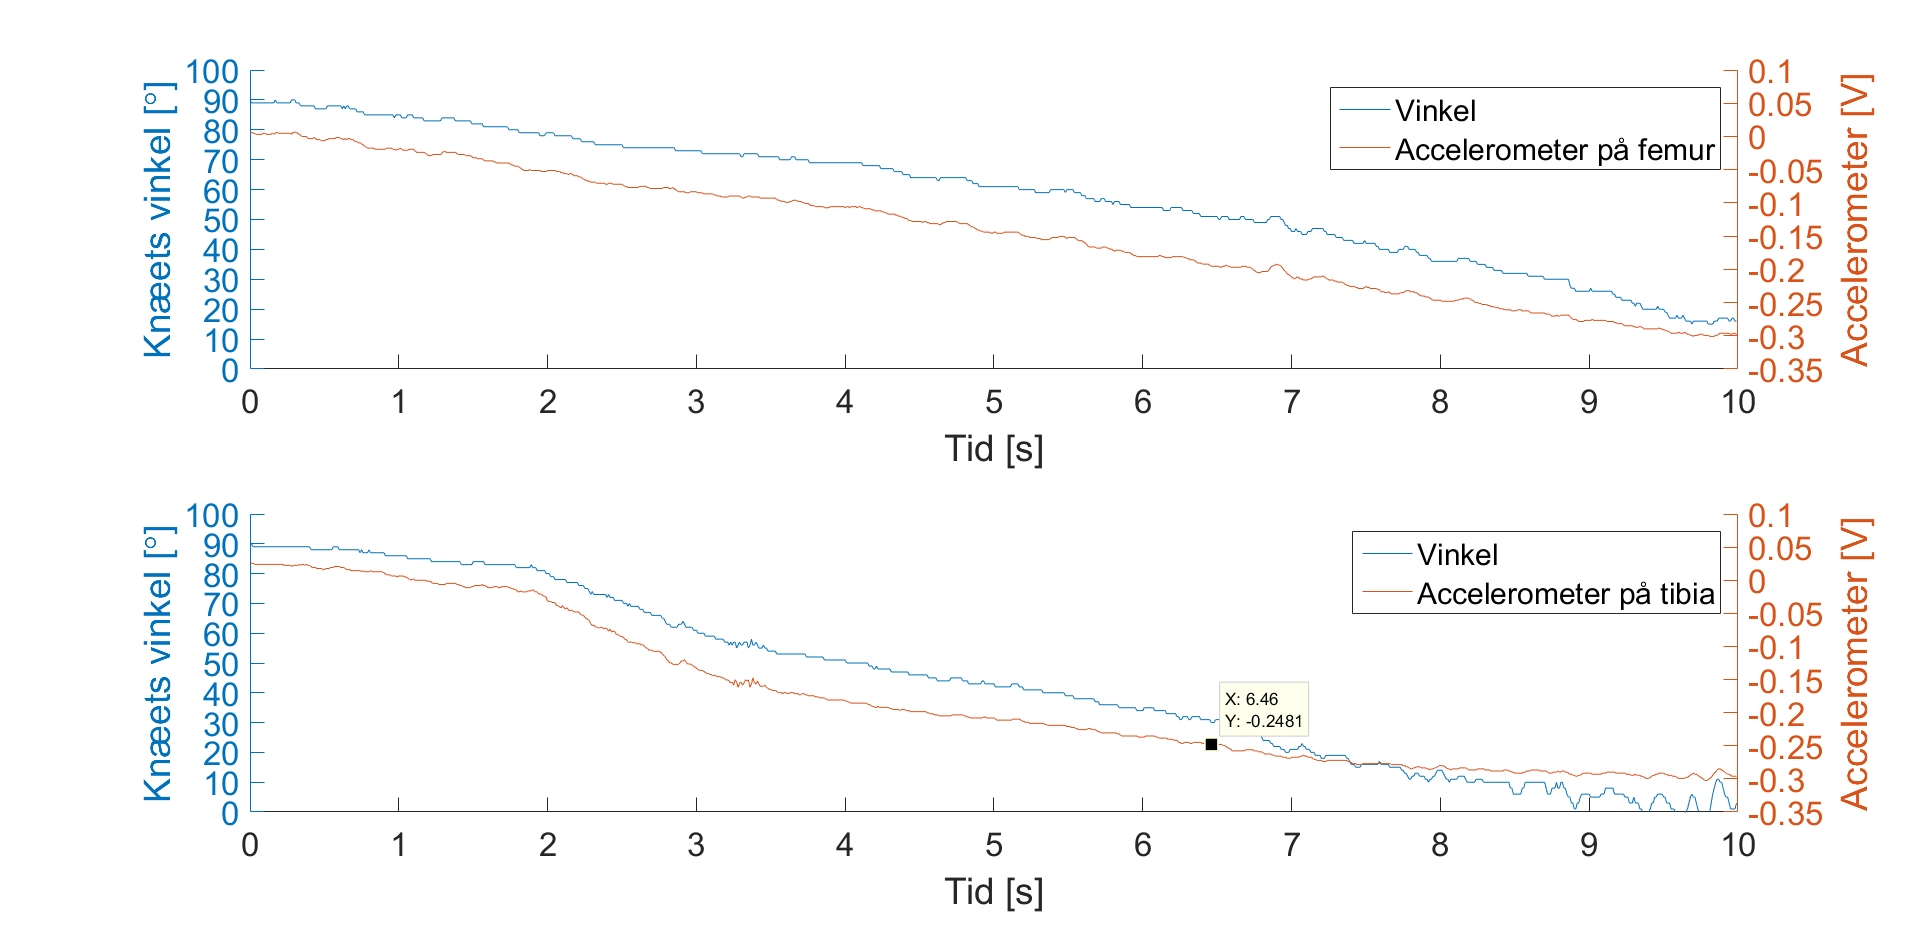
\includegraphics[width=1\textwidth]{figures/vinkel_tibia_femur}
\caption{Test af vinkelberegning. Øverste graf viser vinkel og spænding som funktion af tiden for accelerometret, der skal placeres parallelt med femur. Den nederste graf er for accelerometret, der skal placeres parallelt med tibia. Den blå graf illustrerer vinklen for accelerometrets hældning, hvorved den røde graf illustrerer spændingen for accelerometret.}
\label{fig:test_femur_tibia}
\end{figure}

\noindent
Det ses på \autoref{fig:test_femur_tibia}, at der er en sammenhæng mellem spænding fra accelerometrene og vinklen af accelerometrets hældning. 
Der tages udgangspunkt i \autoref{tab:vinkelinterval_psoc} for omregningen, hvoraf spændingen for hvert accelerometer er opstillet. For de omregnede spændinger svarende til vinkler, for det ene accelerometer, er en afvigelse i forhold til den implementerede spænding og målte spænding vist i \autoref{tab:vinkel_test_afvigelse}.

\begin{table}[H]
\centering
\begin{tabular}{|c|c|c|c|}
\hline
\textbf{Vinkel {[}{$^{\circ}$}{]}} & \textbf{Implementeret spænding {[}V{]}} & \textbf{Målt spænding {[}V{]}} & \textbf{Afvigelse {[}\%{]}} \\ \hline
\multicolumn{1}{|c|}{30}                            & \multicolumn{1}{c|}{-0,2641}                                 & \multicolumn{1}{c|}{-0,2705}                        & \multicolumn{1}{c|}{2,4}                         \\ \hline
\multicolumn{1}{|c|}{50}                            & \multicolumn{1}{c|}{-0,1953}                                 & \multicolumn{1}{c|}{-0,1969}                        & \multicolumn{1}{c|}{0,8}                         \\ \hline
\multicolumn{1}{|c|}{70}                            & \multicolumn{1}{c|}{-0,0960}                                 & \multicolumn{1}{c|}{-0,1008}                        & \multicolumn{1}{c|}{5,0}                         \\ \hline
\multicolumn{1}{|c|}{80}                            & \multicolumn{1}{c|}{-0,0400}                                 & \multicolumn{1}{c|}{-0,0416}                        & \multicolumn{1}{c|}{4,1}                         \\ \hline
\multicolumn{1}{|c|}{90}                            & \multicolumn{1}{c|}{0}                                       & \multicolumn{1}{c|}{0,0064}                         & \multicolumn{1}{c|}{0,6}                         \\ \hline
\end{tabular}
\caption{Tabel over vinkel, den implementerede og målte spændning, og hvoraf en afvigelse er beregnet. Dette er foretaget ud fra det ene accelerometer. Spændingerne og afvigelsen er inddelt efter vinkler på henholdsvis $30$, $50$, $70$, $80$ og $90^{\circ}$. Det fremgår, at afvigelsen er mellem $0,6$ til $5~\%$.}
\label{tab:vinkel_test_afvigelse}
\end{table}

\noindent
Ud fra \autoref{tab:vinkel_test_afvigelse} fremgår en afvigelse mellem $0,6$ og $5~\%$. Resultatet af denne test vurderes til at være sammenlignlig med accelerometret, der skal placeres på tibia, hvorfor en udførelse af denne test ikke forekommer.
Det vurderes herudover, at afvigelsen ikke har den store betydning, da den målte spænding ved for eksempelvis $70^{\circ}$ ligger inden for grænseværdierne mellem $50-70^{\circ}$. 

For at visualisere sammenhængen mellem den samlede vinkel og accelerometrenes spænding, er en test ved hjælp af vinkeltesteren, der ses på \autoref{fig:vinkeltest}, udført.  
Figur \ref{fig:spaending_vinkel_test} visualiserer dette i MATLAB, hvor vinklen er illustreret på den venstre Y-akse, og hvor accelerometrenes spænding er illustreret på den højre Y-akse.

\begin{figure}[H]
\centering
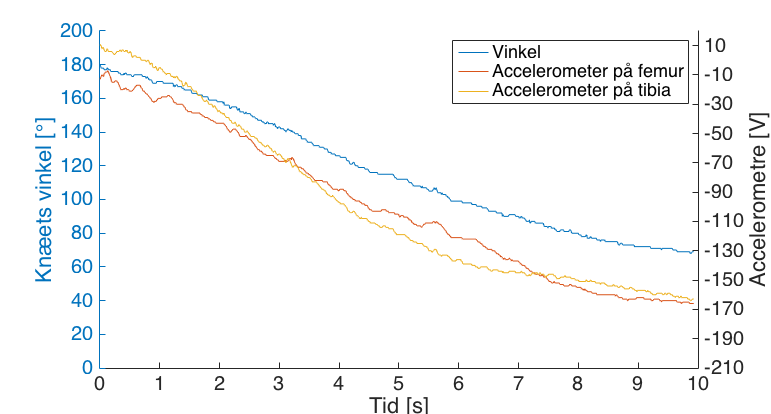
\includegraphics[width=1\textwidth]{figures/spaending_vinkel_test}
\caption{Sammenhængen mellem den samlede vinkel og de to accelerometres spænding som funktion af tiden. Den blå graf, er svarende til den samlede vinkel mellem de to accelerometre, hvor værdierne er illustreret på Y-aksen til venstre i grader. Spændingen målt for de to accelerometre måles i forhold til Y-aksen til højre og er vist ved en rød og gul graf.}
\label{fig:spaending_vinkel_test}
\end{figure}

\noindent
Det fremgar af \autoref{fig:spaending_vinkel_test}, at den samlede vinkel aftager fra $180-70^{\circ}$, herved ses spændingen for de to accelerometre ligeledes faldende.
Derudover illustrerer figuren, at vinklerne virker inden for det forventede arbejdsområde på $90$-$180^{\circ}$, dertil kan vinklen over knæet ligeledes bestemmes under $90^{\circ}$. 
På figuren aflæses, at systemet registrerer en vinkel på $90^{\circ}$, når  accelerometeret på femur giver en spænding på $-0,2191~V$ og accelerometret på tibia giver en spænding på $-0,2336~V$.


For at teste, hvorvidt LED'en på mikrokontrolleren signalerer når en vinkel mellem $90$ og $180^{\circ}$ overskrides, anvendes vinkeltesteren. Vinkeltesteren indstilles til henholdsvis $40^{\circ}$, $100^{\circ}$ og $200^{\circ}$. 
Heraf ses, at LED'en lyser grønt ved de acceptable vinkler mellem $90-180^{\circ}$, og rødt ved vinkler udenfor dette interval. Dette ses på \autoref{fig:mikro_LED}.

\begin{figure}[H]
\centering
\includegraphics[width=1\textwidth]{figures/mikro_LED}
\caption{Mikrokontrollerens LED ses lyse grøn indenfor $90-180^{\circ}$ og lyse rød ved vinkler udenfor.}
\label{fig:mikro_LED}
\end{figure}

\noindent
Ved en overskridelse af grænsen for vinklen, skal det ligeledes visualiseres. 
Der er foretaget en test, hvor accelerometrene er påsat en forsøgsperson, som først overstrækker knæleddet, og derefter udfører en squat-øvelse. 
En visualisering heraf ses af \autoref{fig:vinkeltest_graenser}.

\begin{figure}[H]
\centering
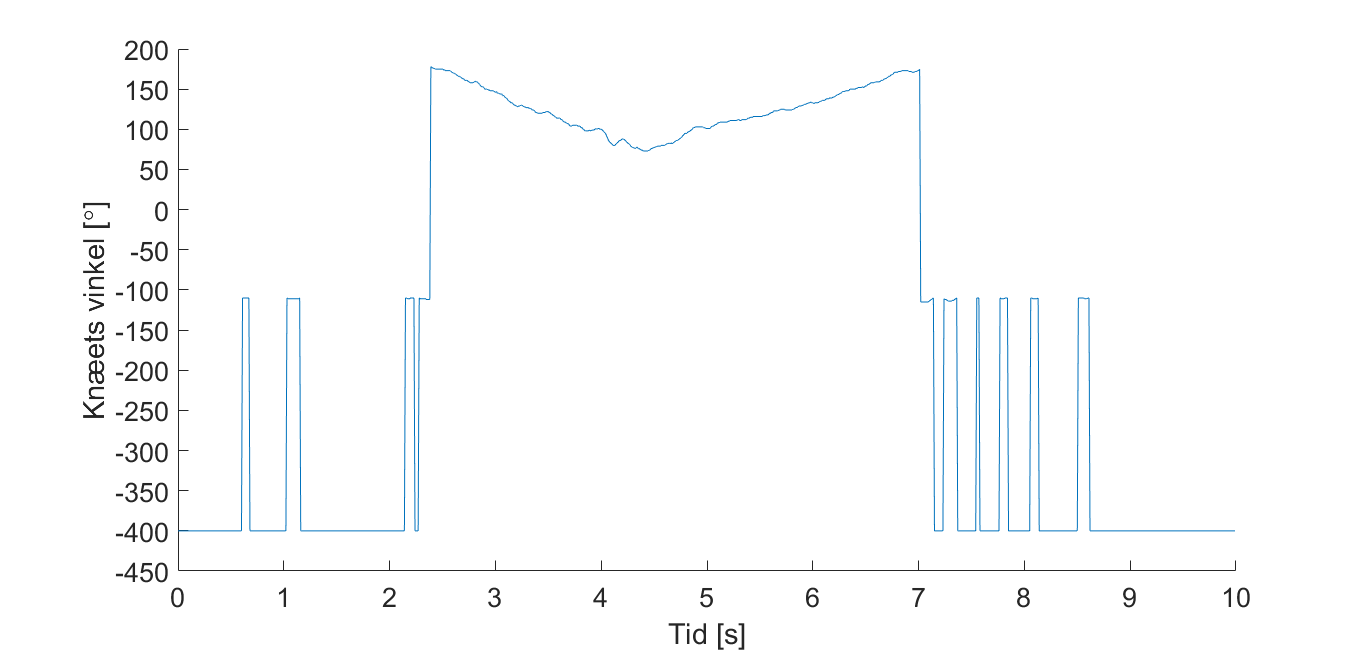
\includegraphics[width=1\textwidth]{figures/vinkeltest_graenser}
\caption{Grafen illustrerer vinklen over knæet under en squat-øvelse. En vinkel under $-100^{\circ}$ symboliserer en overskridelse af $180^{\circ}$ over knæleddet.}
\label{fig:vinkeltest_graenser}
\end{figure}

\noindent
Det ses på \autoref{fig:vinkeltest_graenser}, at forsøgspersonen overstrækker knæleddet de første $2~s$, således begge accelerometre overstiger grænsen på $90^{\circ}$, der tilsammen udgør en vinkel på $180^{\circ}$. 
Dette visualiseres ved en vinkel på $-400^{\circ}$. 
Efter 0,5 sekunder ses en vinkel på $-110^{\circ}$, hvilket er gældende, da det ene accelerometer har haft en spænding svarende til præcis $90^{\circ}$ og har derfor ikke overskredet grænsen. 
Ved squat-øvelsens begyndelse falder vinklen fra $180$ til $73^{\circ}$, hvorefter den stiger til $180^{\circ}$. 
Til slut i målingen ses igen et fald under $-100^{\circ}$, hvilket indikerer, at forsøgspersonen igen overstrækker knæleddet.

\noindent
En yderligere test er foretaget for at undersøge forsinkelsen, og følger samme anvisninger beskrevet i \autoref{sec:lavpas_test}.  
Resultatet af denne test giver en forsinkelse på  $3,6~\mu s$. Dette betragtes ikke som værende af signifikant betydning i forhold til det samlede system, hvorfor denne forsinkelse accepteres.

\vspace{3mm}
\textbf{Opsummering af krav:}
\begin{itemize}
%\item[\text{\sffamily \checkmark}] Skal kunne udregne en samlet vinkel over knæet
\item[\text{\sffamily \checkmark}] Skal kunne udregne knæets vinkel indenfor intervallet $90-180^{\circ}$
\begin{itemize}
\item Dette skal indikeres ved en grøn LED
\end{itemize}
\item[\text{\sffamily \checkmark}] Skal indikere, hvornår knæets vinkel er udenfor intervallet $90-180^{\circ}$
\begin{itemize}
\item Dette skal indikeres ved en rød LED
\item Hvis vinklen for ét accelerometer overstiger $90^{\circ}$, indikeres dette som et output på $-200^{\circ}$, hvortil det andet accelerometers vinkel lægges til de $-200^{\circ}$
\item Hvis vinklen overstiger $90^{\circ}$ for hvert accelerometer, skal dette indikeres som et output på $-400^{\circ}$
\end{itemize}
\end{itemize}